\documentclass[10pt]{article}
\usepackage[utf8]{inputenc}

\title{IF-682 Engenharia de Software e Sistemas}
\author{Artur Cassimiro Alves}
\date{Maio 2019}

\usepackage{natbib}
\usepackage{graphicx}
\usepackage[brazil]{babel}
\usepackage{url}

\begin{document}

\maketitle

\section{Introdução}
A engenharia de software é uma disciplina gerencial e tecnológica que lida com a produção e manutenção sistemática de produtos de software, a disciplina se dedica às teorias, os métodos e as ferramentas para a construção de software profissional com preço, qualidade e tempo de desenvolvimento adequados, utilizando-se os princípios da engenharia.\citep{IntES}

A engenharia de sistemas se preocupa com todos os aspectos do desenvolvimento de sistemas computacionais, incluindo engenharia de hardware, software e processo. Engenharia de software é uma parte específica desse processo mais genérico.\citep{SommervilleES2011}

A disciplina aborda tópicos tais como:

\begin{itemize}
    \item \textbf{Processos de Software}: um conjunto estruturado de atividades, procedimentos, artefatos e ferramentas necessários para o desenvolvimento de um sistema de software;\citep{ProcessosSoftware}
        \begin{figure}[h!]
        \centering
        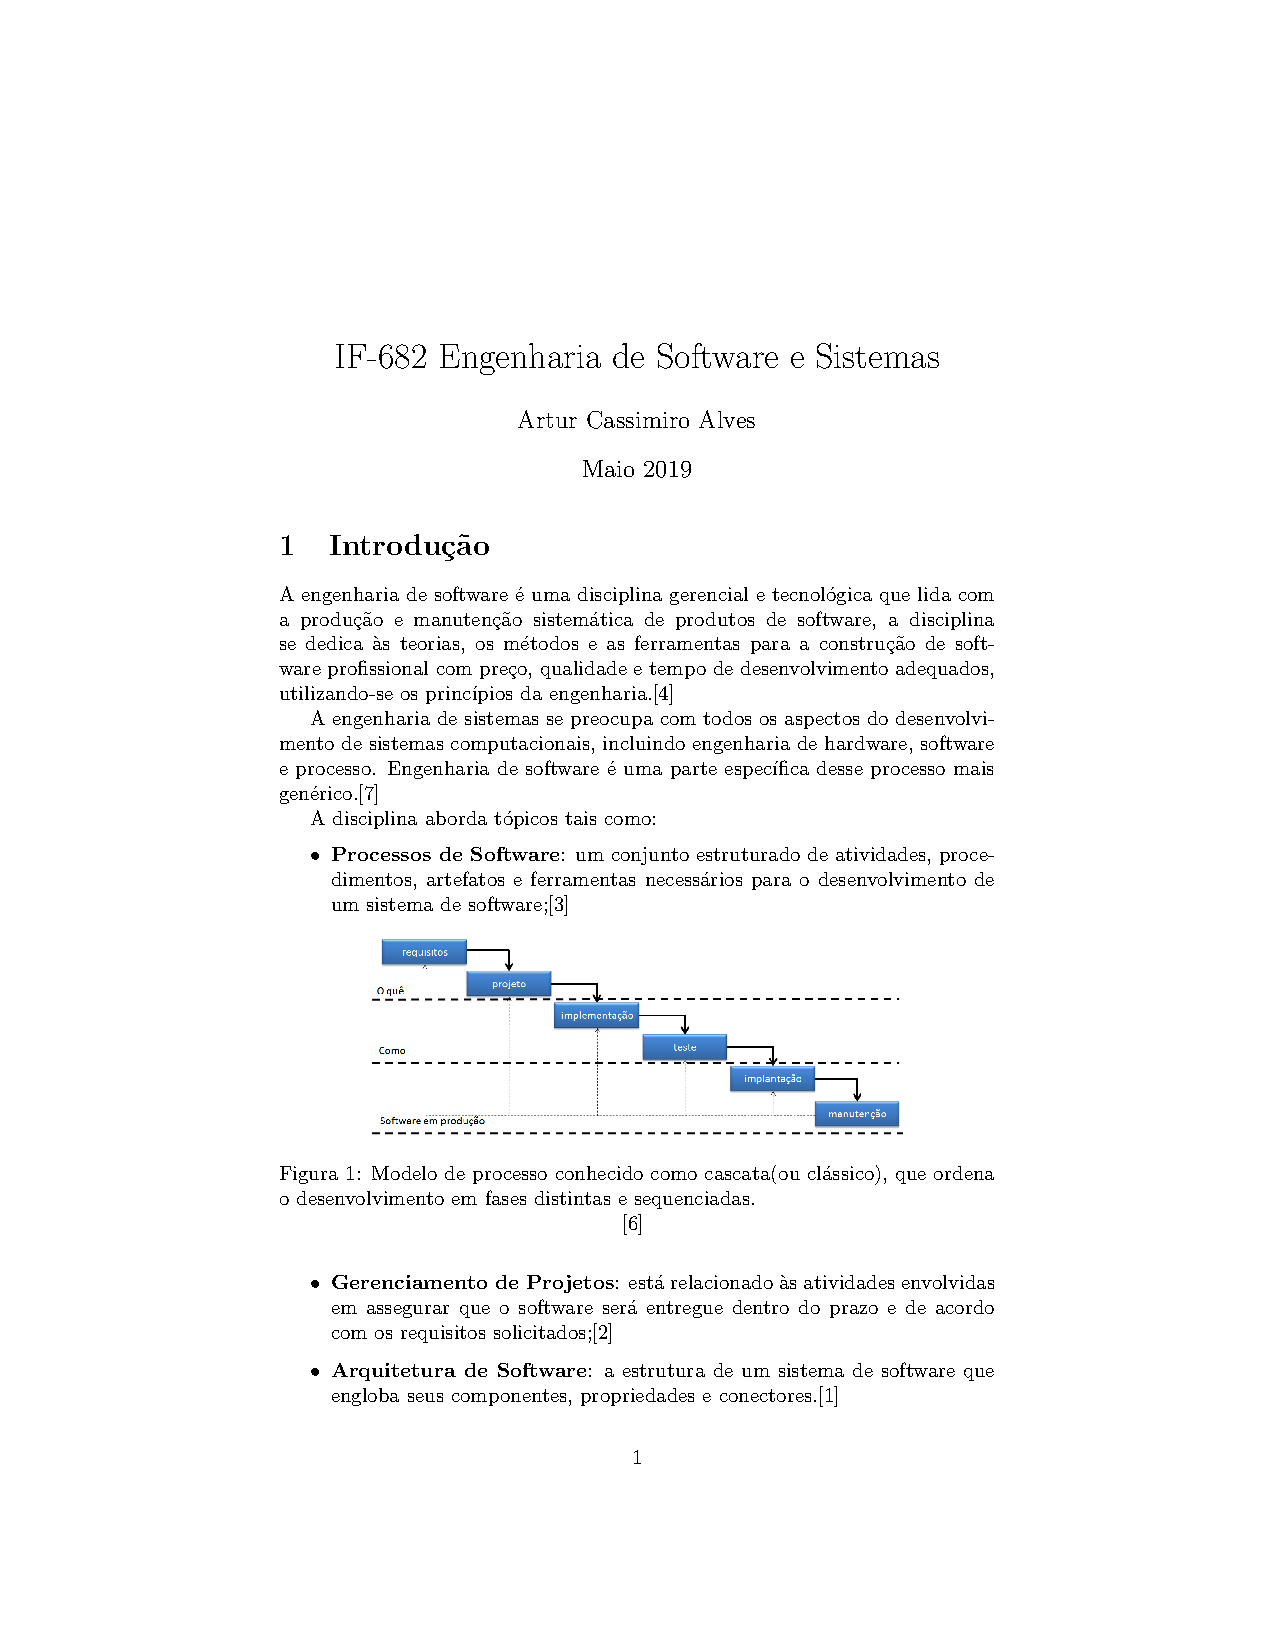
\includegraphics[scale=0.3]{aca7.png}
        \caption{Modelo de processo conhecido como cascata(ou clássico), que ordena o desenvolvimento em fases distintas e sequenciadas.}\citep{Imagem}
        \label{fig:aca7}
        \end{figure}
    
    \item \textbf{Gerenciamento de Projetos}: está relacionado às atividades envolvidas em assegurar que o software será entregue dentro do prazo e de acordo com os requisitos solicitados;\citep{GerenciamentoProjetos}
    
    \item \textbf{Arquitetura de Software}: a estrutura de um sistema de software que engloba seus componentes, propriedades e conectores.\citep{ArquiteturaSoftware}
    
\end{itemize}

\section{Relevância}
A engenharia de software e sistemas está presente no currículo de todos os cursos de graduação do CIn pois essa matéria é de grande importância na gestão de projetos em equipe e possui grande relevância no setor privado.

Devido à sua natureza voltada à aplicação de conhecimentos, a disciplina engenharia de software não cobra muito na questão de matemática, podendo desagradar a alguns universitários, mas a disciplina possui trinta horas de aulas práticas, que geralmente são bem recebidas.  

\section{Relação com outras disciplinas}
Durante a cadeira haverá cobrança altas das habilidades em programação dos alunos para desenvolvimento de um projeto\citep{Cronograma2014}, portanto, as seguintes cadeiras são relevantes à essa disciplina:

\begin{table}[h]
\resizebox{12.1cm}{!}{
\begin{tabular}{l|l}
\textbf{Cadeiras}                      & \textbf{Motivo}                                        \\ \hline
IF-668 Introdução à Computação         & Introdução a conceitos utilizados no desenvolvimento    \\
IF-669 Introdução à Programação        & Introduz os alunos à programação e projetos             \\
IF-672 Algoritmos e Estrutura de Dados & Habilidades de programação, pré-requisito da disciplina \\
IF-673 Lógica para Computação          & Habilidades de programação, pré-requisito da disciplina \\
IF-683 Projeto de Desenvolvimento      & Aplicação da engenharia de software em um projeto                
\end{tabular}}
\end{table}

\bibliographystyle{plain}
\bibliography{aca7}
\end{document}
